\section*{一、预习报告}

\subsection*{1. 实验综述}

通过预习，我了解到弗兰克—赫兹实验是用电子与氩原子的碰撞来研究原子能级。电子能量较小时，主要发生弹性碰撞；当能量达到激发阈值，就可能发生非弹性碰撞，把能量传给氩原子，使它从基态跃迁到激发态。

实验中我们将使用 THQFH-2A 型实验仪和示波器。结合原理图，我先梳理了几个电压的作用：灯丝电压 $U_{F_1F_2}$ 用来加热阴极 $K$，使它发射电子；第一栅压 $U_{G_1K}$ 调节电子流，减小空间电荷的影响；加速电压 $U_{G_2K}$ 使电子获得动能；拒斥电压 $U_{G_2A}$ 则阻止剩余动能不足的电子到达板极 $A$。

\begin{figure}[H]
\centering
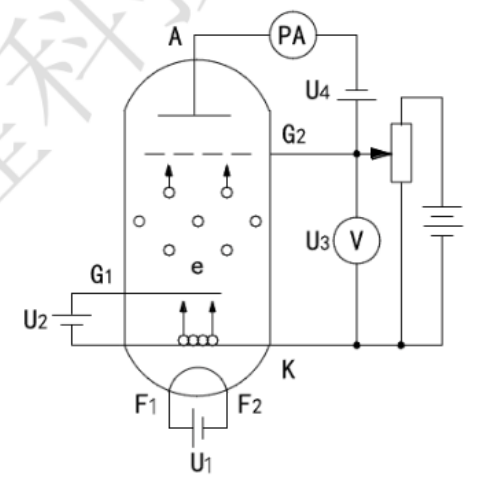
\includegraphics[height=4.0cm]{assets/franck-principle.png}
\caption{弗兰克—赫兹实验原理图}
\end{figure}

其中电流出现峰谷的关键在于电子碰撞后能否克服拒斥电场到达板极。随着加速电压增大，电子经历非弹性碰撞后损失能量，板极电流下降；继续升高电压，电流又回升，从而形成一系列峰谷。同类相邻极值的电压间隔近似等于激发电势 $U_0$，对应的能量差满足

\begin{equation}
eU_0=\Delta E.
\end{equation}

数据处理时，我需要注意测量的是峰之间的电压间隔，而不是第一个峰对应的电压，因为接触电势差会使曲线整体偏移。若一次测量记录了七个峰值电压 $V_1,\ldots,V_7$，就把前三个峰与后三个峰配对，用逐差法求出

\begin{equation}
U_0=\frac{(V_5-V_1)+(V_6-V_2)+(V_7-V_3)}{3\times4}.
\end{equation}

\newpage
这三组配对峰都相隔四个级次，所以求出电压差的平均值后，还要除以 4。实验中计划完成六次自动测量，每次得到一个 $U_0^{(j)}$，最后取平均值：

\begin{equation}
\overline{U_0}=\frac{1}{6}\sum_{j=1}^{6}U_0^{(j)}.
\end{equation}

预备操作是先完成接线、预热、调零，再按实验管的参数标签设置各电压。第一个实验只需要自动测量，先调好示波器量程和外触发，切换到自动方式并按“确认”键启动；约 4 分钟后，用查询键依次读取峰值，将每次的峰值序号和对应加速电压（单位 V）记录在表中，最后求激发电势。第二个实验要求手动测量，将实验仪切换到手动测量方式后，缓慢增大加速电压，每隔 0.5 V、待电流稳定约 4 秒后读数；把电压（V）与电流（nA）成对记录，再绘制电流—电压曲线。

\subsection*{2. 实验目的}

\begin{enumerate}
  \item 通过观察电流的变化，加深对弹性碰撞和非弹性碰撞的理解。
  \item 观察板极电流随加速电压变化的峰谷曲线，理解它为什么能说明原子能级是离散的。
  \item 学习实验仪和示波器的使用方法，并用逐差法测定氩原子的激发电势。
\end{enumerate}

\subsection*{3. 实验重点与难点}

\begin{enumerate}
  \item 接线时，要特别留意加速电压和拒斥电压的极性。通电前先将各电压旋钮逆时针旋到底，检查接线无误后再开机，预热约 15 分钟，并将微电流测量仪调零。
  \item 调出清晰的峰谷曲线是需要关注的重点。灯丝电压过大可能使放大器饱和，过小则峰谷不明显；拒斥电压过小不能有效筛选电子，过大又会使电流太小。因此，我先按实验管上的参数标签设置电压，再观察曲线、适当调整。
  \item 操作时注意保护实验管：灯丝电压不能比参数标签的参考值高出 0.5 V，连续工作不超过 2 小时。如果电流突然剧增，应立即降低加速电压和灯丝电压。实验结束后关闭电源，整理好导线。
\end{enumerate}
